% !TEX TS-program = pdflatex
% !TEX encoding = UTF-8 Unicode

% This is a simple template for a LaTeX document using the "article" class.
% See "book", "report", "letter" for other types of document.

\documentclass[11pt]{article} % use larger type; default would be 10pt

\usepackage[utf8]{inputenc} % set input encoding (not needed with XeLaTeX)

%%% Examples of Article customizations
% These packages are optional, depending whether you want the features they provide.
% See the LaTeX Companion or other references for full information.

%%% PAGE DIMENSIONS
\usepackage{geometry} % to change the page dimensions
\geometry{a4paper} % or letterpaper (US) or a5paper or....
% \geometry{margin=2in} % for example, change the margins to 2 inches all round
% \geometry{landscape} % set up the page for landscape
%   read geometry.pdf for detailed page layout information

\usepackage{graphicx} % support the \includegraphics command and options
\usepackage[rightcaption]{sidecap}

% \usepackage[parfill]{parskip} % Activate to begin paragraphs with an empty line rather than an indent

%%% PACKAGES
\usepackage{booktabs} % for much better looking tables
\usepackage{array} % for better arrays (eg matrices) in maths
\usepackage{paralist} % very flexible & customisable lists (eg. enumerate/itemize, etc.)
\usepackage{verbatim} % adds environment for commenting out blocks of text & for better verbatim
\usepackage{subfig} % make it possible to include more than one captioned figure/table in a single float
% These packages are all incorporated in the memoir class to one degree or another...

%%% HEADERS & FOOTERS
\usepackage{fancyhdr} % This should be set AFTER setting up the page geometry
\pagestyle{fancy} % options: empty , plain , fancy
\renewcommand{\headrulewidth}{0pt} % customise the layout...
\lhead{}\chead{}\rhead{}
\lfoot{}\cfoot{\thepage}\rfoot{}

%%% SECTION TITLE APPEARANCE
\usepackage{sectsty}
\allsectionsfont{\sffamily\mdseries\upshape} % (See the fntguide.pdf for font help)
% (This matches ConTeXt defaults)

%%% ToC (table of contents) APPEARANCE
\usepackage[nottoc,notlof,notlot]{tocbibind} % Put the bibliography in the ToC
\usepackage[titles,subfigure]{tocloft} % Alter the style of the Table of Contents
\renewcommand{\cftsecfont}{\rmfamily\mdseries\upshape}
\renewcommand{\cftsecpagefont}{\rmfamily\mdseries\upshape} % No bold!

%%% END Article customizations

%%% The "real" document content comes below...

\title{SEAG Filters}
\author{Floran, Seppe en Joran}
\date{}
%\date{} % Activate to display a given date or no date (if empty),
         % otherwise the current date is printed 

\begin{document}
\maketitle

\section{Filters}



\section{Low pass}

\section{High pass}


De algemene transfer functie voor een high pass filter ziet er als volgt uit: 
\begin{equation}
H(s) = \frac{s}{s+\omega_c}
\end{equation}
Met $\omega_c$ de cut-off frequentie.
Met behulp van het bilineaire transformatie kunnen we de Z transform vinden:
\begin{equation}
H(z) = H(s)|_{s=\frac{2}{T}\frac{z-1}{z+1}}
\end{equation}
Hierbij is $T$ de sample periode. Dit invullen geeft ons
\begin{equation}
H(z)=\frac{2(z-1)}{(2+T\omega)z-2+T\omega}
\end{equation}
Deze vergelijking kan omgevormd worden naar een differentiaal vergelijking, die dan geïplementeerd kan worden in code.
\begin{equation}
y[n] = \frac{2}{2+T\omega}((x[n]-x[n-1]) - (-2+T\omega)y[n-1] )
\end{equation}
In figure \cite{High Pass bode plot} is een bode plot voor $f_s = 44Khz$ en $\omega = 440$ te zien.
\begin{figure}
	\centering
	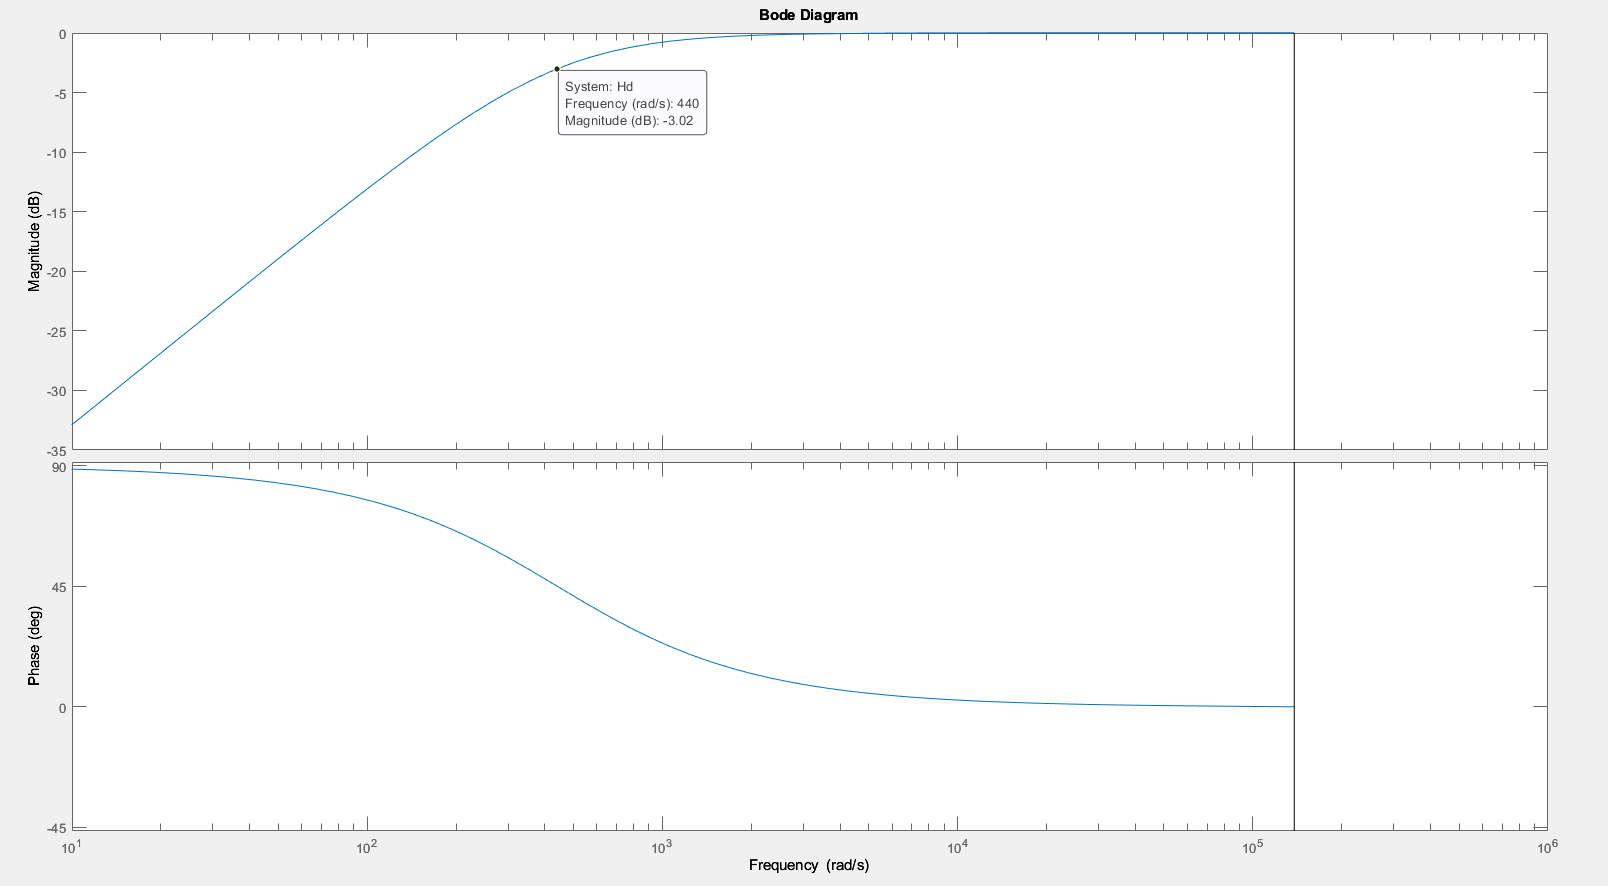
\includegraphics[scale=0.3]{HighPassBodeplot.png}
	\caption{High Pass bode plot}
	\label{Fig:High Pass bode plot}
\end{figure}

\section{Band pass}

\section{Comb feedforward}
Een algemene comb feedfoward kan beschreven worden met volgende differentiaal vergelijking. 
\begin{equation}
y[n] = b_0x[n]+b_Mx[n-M]
\end{equation}
\begin{figure}
	\centering
	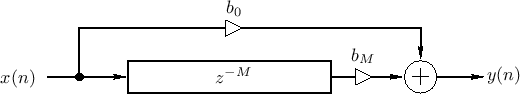
\includegraphics[scale=0.5]{CombFeedfowardBlockDiagram.png}
	\caption{Comb feedforward block diagram}
	\label{Fig:CombFeedforwardBlockDiagram}
\end{figure}

The comb feedforward is een FIR filter.

\section{Comb feedbackwards}
\begin{figure}
	\centering
	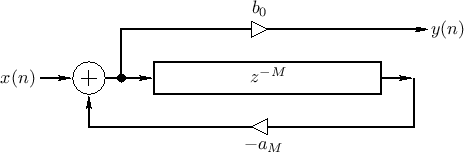
\includegraphics[scale=0.5]{CombFeedbackBlockDiagram.png}
	\caption{Comb feedback block diagram}
	\label{Fig:CombFeedbackBlockDiagram}
\end{figure}

The comb feedbackwards is een IIR filter.

\section{Reverb}

\begin{figure}
	\centering
	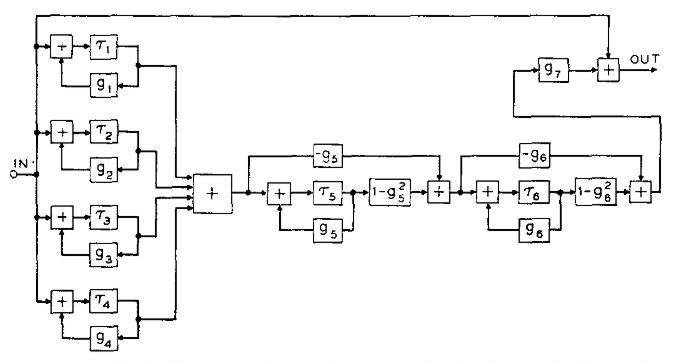
\includegraphics[scale=0.8]{ReverbBlockDiagram.png}
	\caption{Reverb block diagram}
	\label{Fig:ReverbBlockDiagram}
\end{figure}

\section{Flanger}

Flanger wordt geimplementeerd door een comb filter die varieert in delay. \newline
in figure \cite{Fig:FlangerBlockDiagram} wordt het blockschema van een flanger filter gegeven.

\begin{figure}
	\centering
	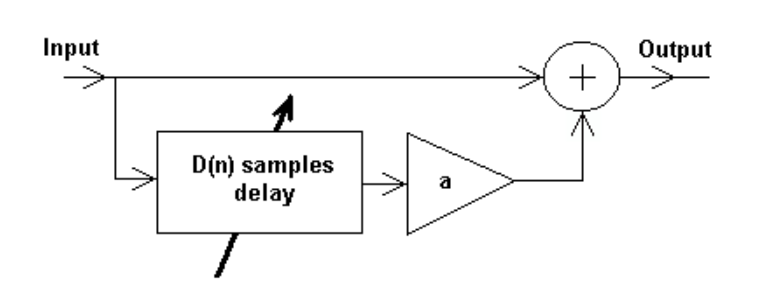
\includegraphics[scale=0.3]{FlangerBlockDiagram.png}
	\caption{Flanger block diagram}
	\label{Fig:FlangerBlockDiagram}
\end{figure}


\section{Chorus}

\cite{Sound Effects}

\section{Auto Wah}

Auto wah is gebaseerd op een bandpass filter, waarvan de cutof frequentie varieert.

\begin{figure}
	\centering
	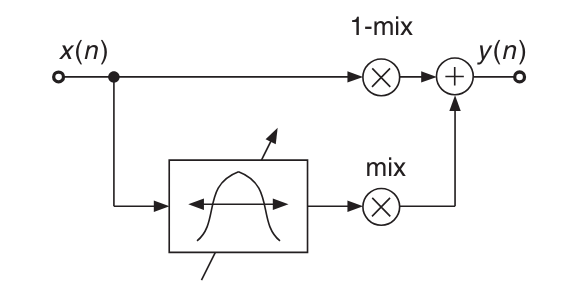
\includegraphics[scale=0.3]{WahBlockDiagram.png}
	\caption{Wah block diagram}
	\label{Fig:WahBlockDiagram}
\end{figure}

\clearpage

\begin{thebibliography}{9}
\bibitem{Sample Data Effect of High-Pass Filters}
David  O. Chin (1981) \emph{Sample Data Effect of High-Pass Filters}
\bibitem{DAFX - Digital Audio Effects}
Xavier Amatrian et al. (2002) DAFX - Digital Audio Effects
\bibitem{Natural Sounding Artificial Reverberation}
M. R. Schroeder (1962) Natural Sounding Artificial Reverbation
\bibitem {Sound Effects}
Sound effects website *insert link*
\end{thebibliography}

\clearpage
\listoffigures

\end{document}
















